Der Raum-Zeit-Pfad ist das Datenmodell, das die geplanten Wege der Agenten beschreibt \cite{book:regele}. Dieses fußt zwar auf das Weltmodell, stellt sich aber nicht als Gitter dar. Die Positionen werden in einem assoziativen Datenfeld, mit dem Schlüssel \(t\), gespeichert. Zusätzlich zu der Definition des Raum-Zeit-Pfades wird in diesem Kapitel kurz erläutert, wie dieser bestimmt wird.

Zu erst wird die Umgebungskarte um zeitlich um \(t\) verschoben und räumlich so, dass die aktuelle Position des Agenten im Zentrum der Umgebungskarte liegt. Dann werden die alten Raum-Zeit-Pfade der anderen Agenten durch die neuen ersetzt. Jetzt kann die Erreichbarkeitskarte entwickelt werden. Um den eigentlichen Weg zu planen, wird nun die letzte Zeitebene der Erreichbarkeitskarte betrachtet. Von den Zellen, die erreichbar sind, also einen Wert halten, wird die ausgesucht, die den kleinsten Entfernung in der Entfernungskarte hat. Von dieser Zelle aus kann man dann den Weg rückwärts durch die Zeit entwickeln. \cite{book:regele}\newline
Nun kann es aber passieren, dass keine Zelle frei ist, oder dass es zu Konflikten mit anderen Agenten kommt. Das wird im Kapitel \ref{chap:konfliktverarbeitung} vertieft.
\begin{figure}[H]
    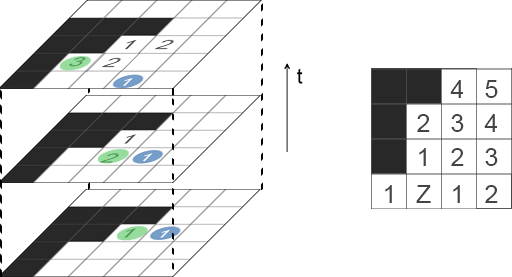
\includegraphics[width=9cm]{images/example_path_planning.png}
    \centering
    \caption{Beispielhafte Wegplanung}
    \label{fig:example_path_planning}
\end{figure}
In Abbildung \ref{fig:example_path_planning} ist die Wegplanung eines Agenten beispielhaft dargestellt. Die Abbildung besteht aus drei Teilen. Zum einen links, die Erreichbarkeitskarte (aus Abbildung \ref{fig:extended_occupancy}), in grün markiert der geplante Weg und rechts ein relevanter Ausschnitt aus der zugehörigen Entfernungskarte (aus Abbildung \ref{fig:distance_localmap}). Die Zelle, die in der Erreichbarkeitskarte in drei Schritten erreichbar ist, besitzt die geringste Entfernung zum globalen Ziel. Diese wird als lokales Ziel markiert. Von hieraus kann nun in der Erreichbarkeitskarte der Weg rückwärts durch die Zeit, hin zur aktuellen Position des Agenten entwickelt werden.